\chapter{\Glsentryfull{mcdp} Representation}
\label{ap:mcdpl}

\newtcolorbox{filebox}[1]{
    colback=white,
    colframe=gray!30,
    fonttitle=\bfseries\sffamily,
    coltitle=black,
    title={#1},
    enhanced,
    attach boxed title to top left={yshift=-2mm, xshift=2mm},
    boxed title style={colback=gray!10},
    breakable
}

\newcommand{\mcdpoutput}[1]{\begin{filebox}{#1}\verbatiminput{mcdpl/#1}\end{filebox}}

The following describes the \gls{mcdp} used in this thesis. This is done in MCDPL, a formal modeling language for the description of \glspl{mcdp}, which is described in \textcite{censi2016Mathematical}. Additionally, catalog files \verb|fleet_bus_count.yaml| and \verb|guidelines.yaml| were created manually using data given by \gls{fps}, and \verb|routing_service.yaml| was created using \gls{bra}.

\begin{figure}[!htbp]
    \centering
    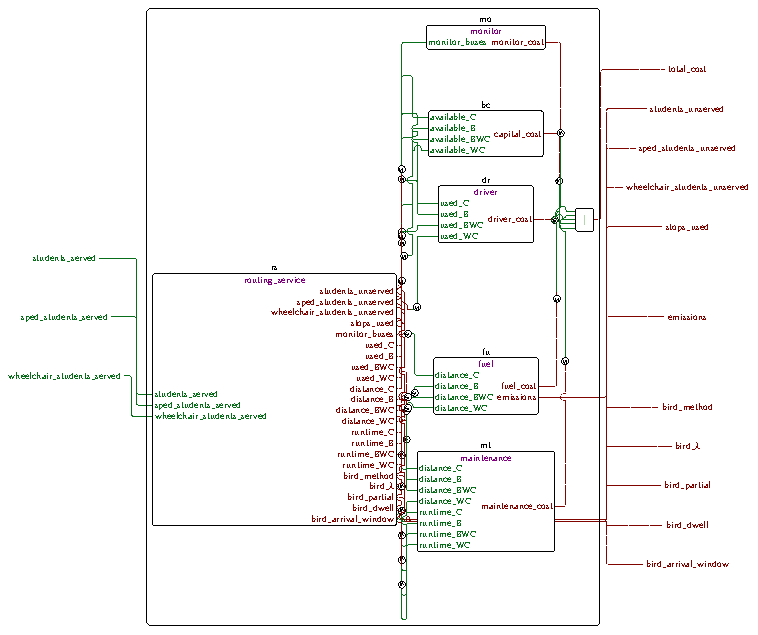
\includegraphics[width=0.99\linewidth, alt={Formal co-design system diagram created from the \glsentryfull{mcdp} showing how routing service inputs, bus capacity, driver, fuel, maintenance, monitor, and \glsentryfull{bird} algorithm requirements connect to functionalities such as total cost, unserved students, stops used, emissions, and accessibility-related service metrics.}]{figures/codesign_diagram.pdf}
    \caption{Formal co-design system diagram generated from the \glsentryfull{mcdp} model, showing how routing service, bus capacity, driver, monitor, fuel, maintenance, and routing algorithm parameters connect to cost, emissions, unserved-student, stop-use, and accessibility-related service metrics.}
    \label{fig:full_mcdp}
\end{figure}

{
\scriptsize
\mcdpoutput{bird\_arrival\_window.mcdp\_poset}
\mcdpoutput{bird\_avg\_speed.mcdp\_poset}
\mcdpoutput{bird\_dwell.mcdp\_poset}
\mcdpoutput{bird\_lambda.mcdp\_poset}
\mcdpoutput{bird\_method.mcdp\_poset}
\mcdpoutput{bird\_partial.mcdp\_poset}
\mcdpoutput{driver.mcdp}
\mcdpoutput{fleet\_bus\_count.mcdp}
\mcdpoutput{fleet.mcdp}
\mcdpoutput{guidelines.mcdp}
\mcdpoutput{maintenance.mcdp}
\mcdpoutput{monitor.mcdp}
\mcdpoutput{routing\_policy.mcdp}
\mcdpoutput{routing\_service.mcdp}
\mcdpoutput{routing\_simple.mcdp\_query.yaml}
\mcdpoutput{routing.mcdp}
}